\documentclass[dvisvgm,tikz,border=4pt]{standalone}\usepackage{amsmath,amssymb}
\usetikzlibrary{arrows.meta,decorations.markings,backgrounds,cd,calc}
\colorlet{c1}{blue!70!black}\colorlet{c2}{red!70!black}\colorlet{c3}{green!45!black}
\tikzset{
 ->-/.style={decoration={markings,mark=at position .55 with {\arrow{Stealth[length=2.4mm]}}},postaction={decorate}},
 ->>-/.style={decoration={markings,mark=at position .5 with {\arrow{Stealth[length=2.4mm]}},mark=at position .6 with {\arrow{Stealth[length=2.4mm]}}},postaction={decorate}},
 every picture/.append style={show background rectangle, background rectangle/.style={fill=white}}
}

\begin{document}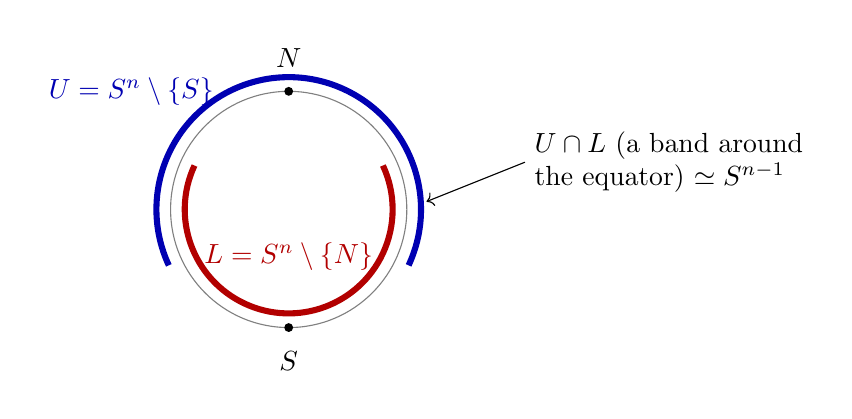
\begin{tikzpicture}
\draw[gray] (0,0) circle(1.5);
\draw[c1,line width=2.2pt] (-25:1.68) arc[start angle=-25,end angle=205,radius=1.68];
\draw[c2,line width=2.2pt] (155:1.32) arc[start angle=155,end angle=385,radius=1.32];
\fill (0,1.5) circle(1.6pt) node[above=5pt]{$N$}; \fill (0,-1.5) circle(1.6pt) node[below=5pt]{$S$};
\node[c1] at (-2.0,1.5){$U=S^n\setminus\{S\}$};
\node[c2] at (0,-0.6){$L=S^n\setminus\{N\}$};
\draw[->] (3.0,0.6) node[right,align=left]{$U\cap L$ (a band around\\ the equator) $\simeq S^{n-1}$} -- (1.75,0.1);
\end{tikzpicture}\end{document}
